
\documentclass[14pt,russian,utf8,nocolumnsxix]{extarticle}
\usepackage{teststyle}

%данные для eskdx

%\ESKDdepartment{факультет КНиТ}
%\ESKDcompany{кафедра Информационно-телекоммуникационных Систем и Технологий}
%\ESKDclassCode{}
%\ESKDtitle{}
%\ESKDdocName{Курсовая работа}
%\ESKDsignature{}
%\ESKDauthor{Ряховский}
%\ESKDchecker{Балабанова}
%\ESKDtitleApprovedBy{}{}
%\ESKDtitleAgreedBy{}{}
%%\ESKDtitleDesignedBy{}{}
%\ESKDcolumnII{1403.210400.213.ПЗКР}
%\ESKDcolumnIX{НИУ <<БелГУ>>}
\begin{document}

%\maketitle
\tableofcontents
\pagebreak

\section*{Введение}
\addcontentsline{toc}{section}{Введение}
В настоящее время, с развитием компьютерных технологий, использование систем автоматического распознавания речи в качестве интерфейса приобретает все большую популярность. Однако, создание таких систем является нетривиальной задачей. Это связано прежде всего с тем, что каждая реализация произнесенного слова может отличаться от любой другой по целому ряду признаков. Например, по частоте или громкости. Также анализируемый речевой сигнал может быть растянут или сжат по времени относительно образца, с которым производится сравнение. Именно для минимизации временных различий служит рассмотренный в данной работе алгоритм.

\pagebreak
\section{Теория распознавания речи}
\subsection{Способы распознавания речи}
Выделяют несколько основных способов распознавания речи:


Распознавание отдельных команд.
\begin{itemize}
\item Суть технологии: раздельное произнесение и последующее распознавание слова или словосочетания из небольшого заранее заданного словаря.

\item Техническая реализация: точность распознавания ограничена объемом заданного словаря. При соблюдении этого условия данная технология позволяет достичь самой высокой достоверности распознавания.

\item Применение: в настоящее время наиболее ярким примером использования технологии распознавания отдельных команд в коммерческих приложениях является голосовая навигация по сайтам.
\end{itemize}

Распознавание по грамматике
\begin{itemize}
\item Суть технологии: распознавание фраз, соответствующих определенным заданным правилам (грамматике).

\item Техническая реализация: для задания грамматик используются стандартные XML-языки (VoiceXML), обмен данными между системой распознавания и приложением, как правило, осуществляется по протоколу MRCP.

\item Применение: технология распознавания по грамматике широко применяется в системах голосового самообслуживания (СГС).
\end{itemize}

Поиск ключевых слов в потоке слитной речи.
\begin{itemize}
\item Суть технологии: распознавание отдельных участков речи.

\item Техническая реализация: в этом случае речь может быть как спонтанной, так и соответствующей определённым правилам. Произнесенная речь не полностью преобразуется в текст - в ней автоматически находятся лишь те участки, которые содержат заданные слова или словосочетания.
\end{itemize}

Распознавание слитной речи на большом словаре (LVCSR — large vocabulary continuous speech recognition).
\begin{itemize}
\item Суть технологии: эта технология наиболее близка к мечте человека о взаимодействии человека и машины – все, что сказано, дословно преобразуется в текст. Поэтому иногда эта технология так и называется STT – speech to text.

\item Техническая реализация: задача полноценного распознавания слитной речи не решена нигде в мире, однако, достоверность распознавания уже достаточно высока для использования технологии на практике.

\itemПрименение: потенциальная сфера применения технологии в коммерческих целях довольно широка.
\end{itemize}

В данной работе реализован способ распознавания отдельных речевых команд.

\subsection{Ограничения систем распознавания}
Задача распознавания речи состоит в восстановлении по звуковому сигналу слова естественного языка (из ограниченного словаря), произнесением которогоя является звуковой сигнал. Она обычно решается путем задания эталонов слов словаря и последующего сравнения звуковых сигналов с этими эталонами. Звуковой сигнал представляет из себя целочисленный вектор значений звукового давления, измеренного в равноотстоящие друг от друга моменты времени. Мощность пространства звуковых сигналов огромна. Для решения задачи распознавания обычно сначала равномерно разбивают сигнал на окна одинаковой длины. Окна преобразуют из временной области в частотную (например, с помощью преобразования Фурье), чтобы близость окон относительно простых метрик (типа Евклидовой) соответствовала близости участков сигнала "на слух". Затем решается задача нахождения соответствия между окнами звукового сигнала и окнами эталонов словаря. Сложность последней задачи заключается в том, что различные участки звукового сигнала в различных произнесениях одного и того же слова отличаются разной степенью сжатия или растяжения (вовсе не пропорционального). Для решения задачи нахождения соответствия между окнами сигналов традиционно используются методы динамического программирования. Создание компьютерных систем распознавания речи связано со множеством объективных трудностей, накладывающих на подобные системы искусственного интеллекта ряд ограничений.
Предельные возможности компьютера по распознаванию речи связаны прежде всего с тем, что человек, которого можно взять за эталон распознающей системы, распознает осмысленную речь, а компьютеру в полной мере это не дано. Компьютер принципиально не может с требуемой надежностью исправлять ошибки и неоднозначности распознавания, используя синтаксическую и семантическую связь слов предложения. Вместо этого в современных системах используется статистическая модель, задающая связь последовательных троек слов предложения. Кроме того человек использует зачастую дополнительную, незвуковую информацию. Самым ярким примером здесь может служить так называемое <<чтение по губам>>, которому могут обучиться глухие люди. Известно, что в шумной обстановке человеку легче распознать речь, если он следит за губами говорящего. Человек воспринимает речь объемно, что позволяет ему производит шумоочистку и пространственное выделение сигнала более качественно, чем ЭВМ.
Дополнительно картина осложняется тем, что все известные алгоритмы распознавания речи являются дикторозависимыми. После настройки на голос одного диктораа распознающие системы дают удовлетворительные результаты распознавания для этого типа голоса, но хуже работают на других голосах. Надежность распознавания речи человеком, напротив, не зависит от типа голоса диктора.\cite{mazurenko}

\subsection{Способы описания речевых сигналов}

При распознавании речевых сигналов, как правило, оперируют не с исходным речевым сиrналом, получаемым на выходе микрофона, а с так называемым описанием речевоrо сигнала, экономно представляющим речевой сигнал и содержащим информацию о том, что говорится. 
Обычно принято описывать (задавать) речевой сигнал последовательностью $X_{I}=\{x_{1},x_{2},\dots,x_{i},\dots,x_{I}\}$ из элементов $x_{i}$, которые являются отсчетами векторной функции $x(t)$ в дискретные равноотстоящие моменты времени $t_{i}=i\Delta T$ с шагом $\Delta T$, принимаемым равным, например, 15 мс. Тоrда $I$ это длина речевого сигнала в дискретном равномерном времени с шагом $\Delta T$. Вообще говоря, может быть использовано и неравномерное время с изменяющимся шагом $\Delta T$, выбираемым, например, из диапазона 8-25 мс. В любом случае, однако, речевой сиrнал будет представляться последовательностью $X_{I}$ , из элементов $x_{i}$. 
Последовательности $X_{I}$ получают в результате предварительной обработки речевоrо сигнала на выходе микрофона, чем существенно сокращается объем информации. Так, исходный речевой сигнал, который характеризуется объемом 200000 бит/с, как правило, описывается существенно меньшим объемом информации --- от 9600 до 600 и менее бит/с, однако все еще сохраняющим существенную информацию о том, что говорится, чтобы по ней отвечать на вопросы о распознаваемом классе. 
Вопросам предварительной обработки речевоrо сигнала посвящено oгpoмнoe количество работ. Несмотря на многочисленность предложений все они сводятся к тому, что элементы речи описываются величинами, представляющими в той или иной форме мгновенные передаточную характеристику речевоrо тракта и параметры источников eгo возбуждения. Поскольку эти величины изменяют свои значения сравнительно медленно в процессе произнесения речи, то для подробноrо описания речевых сиrналов вполне достаточно ограничиться временной дискретизацией элементов с шаrом $\Delta T=$ 15 мс. 
Чаще Bcero элементами речи $x_{i}$ выступают мгновенный амплитудный спектр речи или мгновенная автокорреляционная функция, мrновенный продольный профиль акустической трубы речевоrо тракта, мгновенные значения параметров линейной системы, представляющей речевой тракт, мгновенные значения системы двоичных признаков, характеризующих звуки по месту и способу образования и т. п. Для многих описаний речевоrо сигнала могут быть указаны взаимнооднозначные преобразования, позволяющие переходить от одного описания к друrому. 
Элементы $x_{i}$ могут содержать компоненты, описываемые разнородными физическими величинами. Например, наряду с компонентами, представляющими форму амплитудноrо спектра речи или передаточную характеристику речевоrо тракта, могут быть компоненты, характеризующие интенсивность элемента, способ ero образования (с участием голоса или только шума), относительную частоту основного тона и т. п. 
Последовательности $X_{I}$, элементов $x_{i}$ получают, анализируя речевой сигнал на интервале (окне) анализа продолжительностью $\Delta T'\geq \Delta T$ и перемещая это окно вдоль оси времени с шаrом $\Delta T$. Таким образом, интервалы анализа либо соприкасаются, либо перекрываются. \cite{vincuk}

\subsection{Психофизические единицы измерения}
Психоакустика - наука о природе восприятия звука. 
Органы слуха выполняют двойное кодирование звука, как спектральное, так и временное.
В отдельном звуке восприятие выделяет пять основных свойств. Это громкость, тембр, высота, продолжительность и пространственная локализация. При этом громкость можно соотнести с амплитудой колебаний, тембр - с формой волны, высоту - с частотой колебаний.

Использование психофизических единиц для описания речевых сигналов позволяет приблизиться к механизмам человеческого восприятия речи, которые, во многом, являются образцом для систем автоматического распознавания. В данной работе для описания характеристик речевых сигналов используется единица высоты звука мел.

Мел --- психофизическая единица высоты звука, применяется главным образом в музыкальной акустике. Количественная оценка звука по высоте основана на статистической обработке большого числа данных о субъективном восприятии высоты звуковых тонов. Результаты исследований показывают, что высота звука связана главным образом с частотой колебаний, но зависит также от уровня громкости звука и его тембра. Звуковые колебания частотой 1000 Гц при эффективном звуковом давлении $2 \cdot 10^{-3}$ Па (то есть при уровне громкости 40 фон), воздействующие спереди на наблюдателя с нормальным слухом, вызывают у него восприятие высоты звука, оцениваемое по определению в 1000 мел. Звук частоты 20 Гц при уровне громкости 40 фон обладает по определению нулевой высотой (0 мел). Зависимость нелинейна, особенно при низких частотах (для «низких» звуков).
Преобразовать значение частоты звука (Гц) в значение высоты (мел) можно по формуле: $m=1125\ln(1+f/700)$
\begin{figure}[H]
\centering
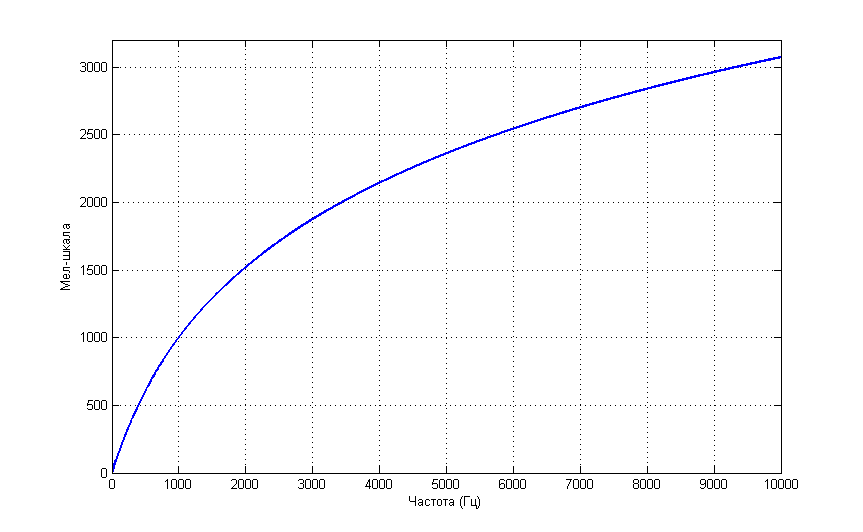
\includegraphics[width=120mm]{mel-scale.png}
\caption{Зависимость воспринимаемой высоты звука от его частоты}
\label{mel-scale}
\end{figure}

\subsection{Кепстральный анализ}
Кепстральный анализ применяют для сигналов, представляющих собой свертку двух временных функций, причем таких, что после преобразования их в спектр они образуют неперекрывающиеся на оси q импульсы.

Пример. Задан сигнал $s_{вых}(t)$ на выходе линейного тракта. Требуется определить некоторую информацию о входном сигнале $s_{вх}(t)$ и самом тракте, например, о его импульсной характеристике $h(t)$.

Выходной сигнал определяется сверткой $s_{вых}(t)=s_{вх}(t)\otimes h(t)$.


Т.к. $S_{вых}(\omega)=S_{вх}(\omega)H(\omega)$ в линейном тракте, то после логарифмирования получаются функции $\ln S_{вх}^{2}(\omega)$ и $\ln H^{2}(\omega)$, а на выходе сумма кепстров $C_{s}(q)$ и $C_{h}(q)$.

Таким образом, кепстральный анализ позволяет развернуть речевой сигнал, и получить информацию о состоянии артикуляционного аппарата, которая недоступна в частотной или временной области.



\pagebreak
\section {Реализованные алгоритмы}
\subsection{Алгоритм нахождения мел-частотных кепстральных коэффициентов}


Запишем исходный речевой сигнал как  
\[
	x[n], \; \; 0 \leq n < N 
\]

Получим спектр сигнала, используя ДПФ
\[
	X_{a}[k]=\sum_{n=0}^{N-1}{x[n]e^{\frac{-2\pi i}{N}kn}}, \; \;  0 \leq k < N
\]

Определим оконные функции. В данном случае использованы треугольные окна, равномерно расположенные относительно мел-шкалы
\[
	H_{m}=
	\begin{cases}
		0,&k<f[m-1]\\ 
		\frac{(k-f[m-1])}{(f[m]-f[m-1])},&f[m-1] \leq k < f[m]\\ 
		\frac{(f[m+1]-k)}{(f[m+1]-f[m])},&f[m] \leq k \leq f[m+1]\\ 
		0,&k > f[m+1]
\end{cases}
\]

Граничные частоты $f[m]$ получены из равенства
\[
	f[m]=(\frac{N}{F_{s}})B^{-1}(B(f_{1})+m\frac{B(f_{h})-B(f_{1})}{M+1})
\]

где $B(f)$ --- операция перевода значений частоты в мел-шкалу
\[
	B(f)=1125\ln(1+f/700)
\]

Соответственно, обратная операция
\[
	B^{-1}(b)=700(exp(b/1125)-1)
\]

\begin{figure}[H]
	\begin{multicols}{2}
		\hfill
		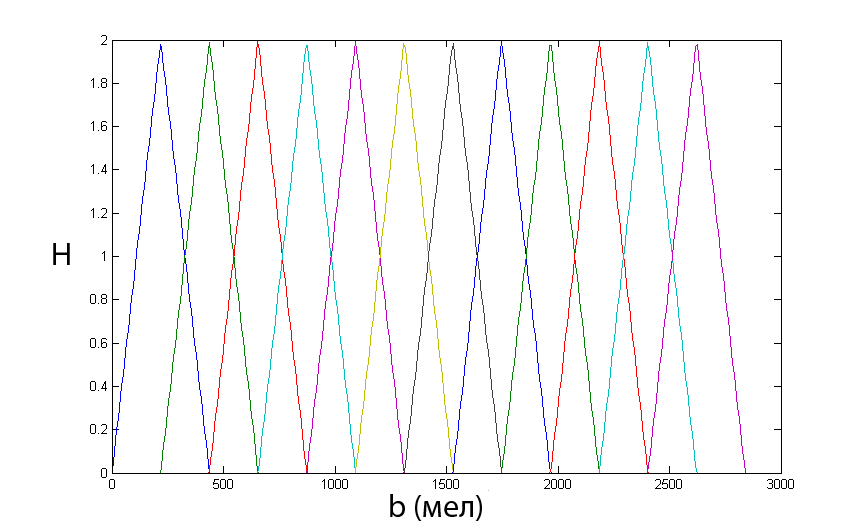
\includegraphics[width=85mm]{graph-3.png}
			%\hfill
			\caption{Окна (мел-шкала)}
			\label{wind-mel}
			%\hfill
		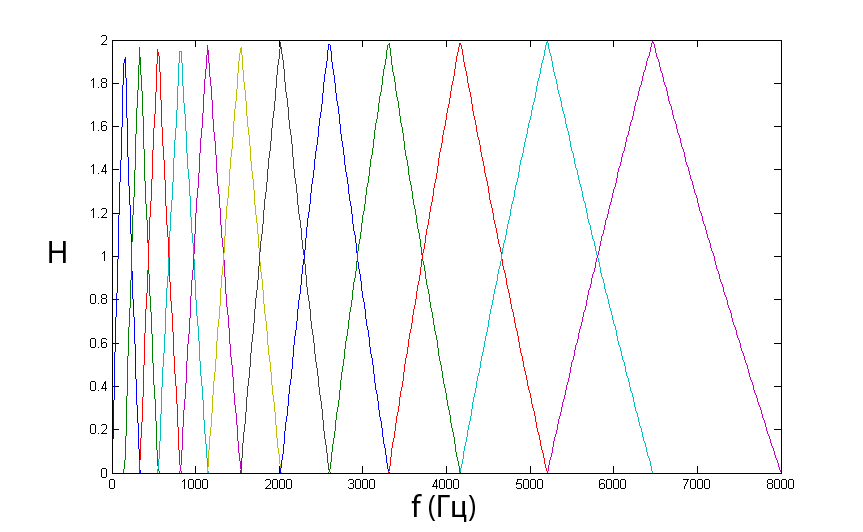
\includegraphics[width=85mm]{graph-4.png}
			%\hfill
			\caption{Окна (частотная шкала)}
			\label{wind-hz}
	\end{multicols}
\end{figure}

Вычислим значения энергии сигнала для каждого окна
\[
	S[m]=ln(\sum_{k=0}^{N-1}{|X_{a}[k]|^{2}H_{m}[k])}, \; \; 0\leq m<M
\]

К полученным значениям применим ДКП
\[
	c[n]=\sum_{m=0}^{M-1}{S[m]cos(\pi n(m+1/2)/M)}, \; \; 0\leq n < M
\]

Полученные в результате значения, а также их изменения во времени, используются в дальнейшем как описание речевого сигнала.
\pagebreak

\subsection{Алгоритм сравнения речевых сигналов с применением динамического программирования (DTW)}

Алгоритм динамического трансформирования времени (DTW) вычисляет оптимальную последовательность трансформации (деформации) времени между двумя временными рядами. Алгоритм вычисляет оба значения деформации между двумя рядами и расстоянием между ними. 


Предположим, что есть две числовые последовательности $A= a_{1}, a_{2}, \dots, a_{I}$ и $B=b_{1}, b_{2}, \dots, b_{J}$. Длина двух последовательностей может быть различной.

Временные различия между A и B могут быть описаны с помощью некоторой последовательности $c=(i,j)$:
\[
	F=c(1),c(2)\dots,c(k),\dots,c(K)
\]
где $c(k)=(i(k),j(k))$.
Данная последовательность представляет собой функцию, которая позволяет отобразить временную ось A на временной оси B. Назовем ее функцией деформации. \cite{sakoechiba}

\begin{figure}[H]	
	\centering
	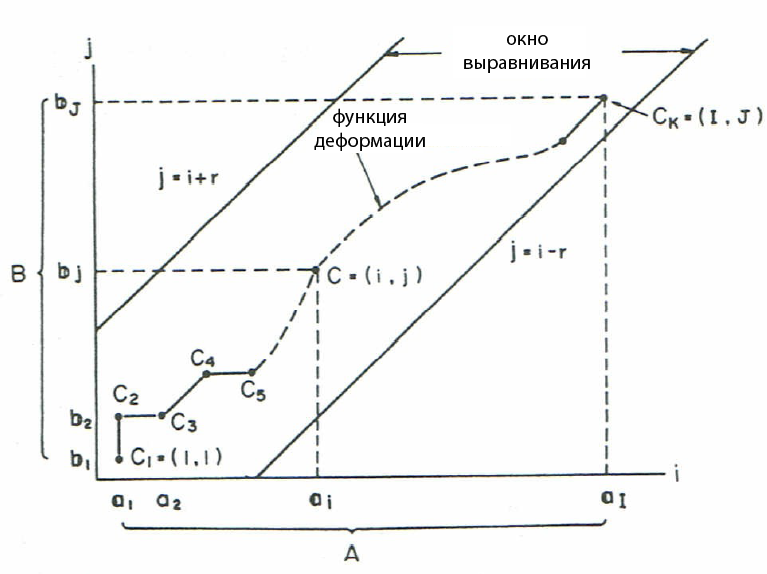
\includegraphics[width=120mm]{sakoe1.png}			
	\caption{Функция деформации и окно выравнивания}
	\label{sakoe1}
\end{figure}

Алгоритм начинается с расчета локальных расстояний между элементами двух последовательностей. Самый распространенный способ для вычисления расстояний является метод, рассчитывающий модуль разности между значениями двух элементов (Евклидова метрика). В результате получаем матрицу расстояний, имеющую n строк и m столбцов общих членов:
\[
d(c)=d(i,j)=|a_{i}-b_{j}|, i=1..I, j=1..J
\]

Взвешенная сумма значений метрик в точках, принадлежащих функции деформации F
\[
E(F)=\sum_{k=1}^{K}{d(c(k))\cdot w(k)}
\]
(где $w(k)$ - неотрицательный весовой коэффициент) является мерой доброкачественности функции F. Она принимает минимальное значение, когда функция F оптимально выравнивает временные различия между A и B. Минимальное остаточное расстояние между A и B, которое остается после устранения временных различий, может служить мерой различия речевых последовательностей A и B
\[
D(A,B)=min_F\left[\frac{\sum_{k=1}^{K}{d(c(k))\cdot w(k)}}{\sum_{k=1}^{K}{w(k)}}\right]
\]


Существует три условия, налагаемых на DTW алгоритм для обеспечения быстрой конвергенции:

\begin{enumerate}
 \item Монотонность – путь никогда не возвращается, то есть: оба индекса, i и j, которые используются в последовательности, никогда не уменьшаются. 

 \item Непрерывность – последовательность продвигается постепенно: за один шаг индексы i и j, увеличиваются не более чем на 1.

 \item Предельность – последовательность начинается в (1,1) и заканчивается в (I,J).
 \end{enumerate}

Практическая реализация данного алгоритма представляет собой нахождение значения нормированного расстояния
\[
D(A,B)=\frac{1}{N}g_{K}(c(K))
\]
где $g_{k}(c(k))$ можно найти из уравнения:
\[
g_{k}(c(k))=\min_{c(k-1)}[g_{k-1}(c(k-1))+d(c(k))\cdot w(k)]
\]

Начальное условие:
\[
g_{1}(c(1))=d(c(1))\cdot w(1)
\]

Из ограничений следует, что $c(1)=(1,1)$,
\[
g(i,j)=\min \left[ \begin{matrix} g(i,j-1)+d(i,j) & \\ g(i-1,j-1)+2d(i,j) &\\ g(i-1,j)+d(i,j) &\end{matrix} \right].
\]

В данном случае нормированное расстояние можно записать как
\[
D(A,B)=\frac{1}{N}g(I,J), \text{где } N=I+J.
\]
\begin{figure}[H]	
	\centering
	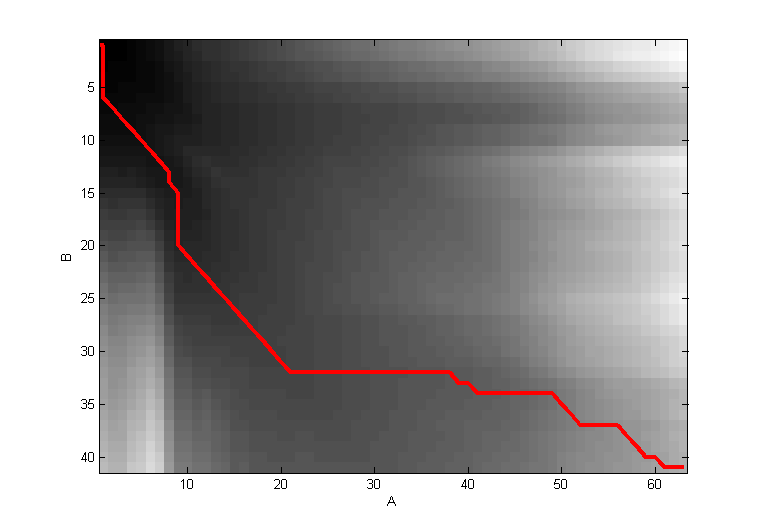
\includegraphics[width=120mm]{d_matrix.png}			
	\caption{Пример нахождения функции деформации}
	\label{d_matrix1}
\end{figure}

Эксперименты проводились для словаря из 10 слов (цифры от 0 до 9). Одним диктором было записано 100 повторений для сравнения (по 10 для каждого в словаре).


С помощью данного алгоритма производится сравнение анализируемого сигнала с сохраненными в памяти компьютера эталонами. В результате выбирается пара с минимальной дистанцией и делается вывод о соответствии сигнала слову из словаря. Пример результата сравнения можно видеть на рис. \ref{distances_4} (Меньшее значение дистанции означает большее сходство).

\begin{figure}[H]	
	\centering
	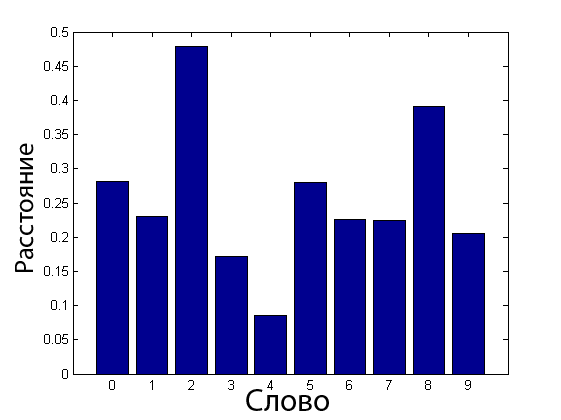
\includegraphics[width=120mm]{distances_4.png}			
	\caption{Диаграмма расстояний для слова <<четыре>>}
	\label{distances_4}
\end{figure}

В результате, на 100 повторений было обнаружено 2 ошибки распознавания, что позволяет говорить о достаточной точности выбранного алгоритма. На рис. \ref{dist_err_8} показана диаграмма расстояний для ошибочно распознанного слова <<восемь>>

\begin{figure}[H]	
	\centering
	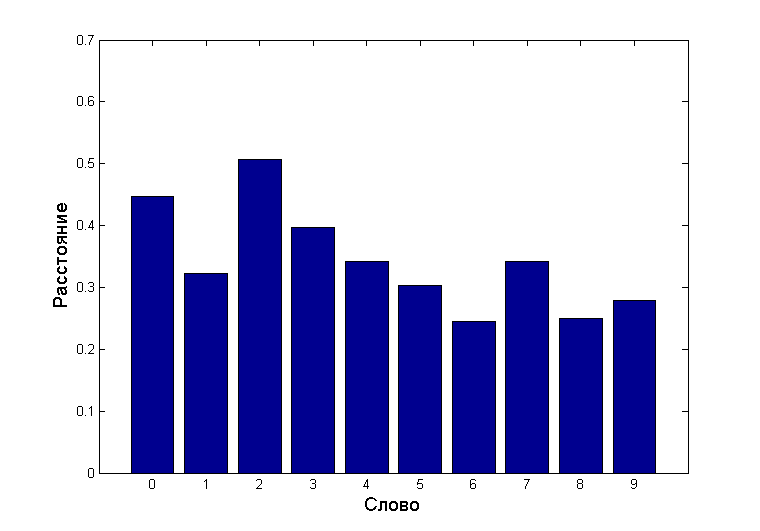
\includegraphics[width=120mm]{err_8.png}			
	\caption{Диаграмма расстояний для ошибочно распознанного слова <<восемь>>}
	\label{distances_4}
\end{figure}


\pagebreak
\subsection{Листинг программы на языке MATLAB}

\begin{lstlisting}
function out = mfcc(sig,nfilt,wlen,woverlap) % MFCC calculation
% sig = input signal
% nfilt = number of coefficients
% wlen = window width
% woverlap = window increment
%
%

if nargin <4
    woverlap=128;
    if nargin <3
        nfilt=24;
        if nargin <2
            wlen=256;
        end
    end
end

bank=melbankm(nfilt,wlen,16000,0,0.5,'m'); 
bank=full(bank); 
bank=bank/max(bank(:)); 
 
dctcoef=zeros(nfilt/2,nfilt);

for k=1:(nfilt/2)
  n=0:nfilt-1; 
  dctcoef(k,:)=cos((2*n+1)*k*pi/(2*nfilt)); 
end 
 
 
w = 1 + 6 * sin(pi * (1:nfilt/2) ./ (nfilt/2)); 
w = w/max(w); 
 

xx=double(sig); 
xx=filter([1 -0.9375],1,xx); 
 

xx=enframe(xx,wlen,woverlap); 
 
m=zeros(size(xx,1),size(dctcoef,1));

for i=1:size(xx,1) 
  y = xx(i,:); 
  s = y' .* hamming(wlen); 
  t = abs(fft(s)); 
  t = t.^2; 
  c1=dctcoef * (log(bank * t(1:(wlen/2+1)))); 
  c2 = c1.*w'; 
  m(i,:)=c2'; 
end 
 

dtm = zeros(size(m)); 
for i=3:size(m,1)-2 
  dtm(i,:) = -2*m(i-2,:) - m(i-1,:) + m(i+1,:) + 2*m(i+2,:); 
end 
dtm = dtm / 3; 
 
 
out = [m dtm]; 

out = out(3:size(m,1)-2,:); 

\end{lstlisting}

\begin{lstlisting}
function [Dist, p, q] = dtw( siga, sigb )
%DTW Dynamic time warp

S1=siga';
S2=sigb';
    ES1 = sqrt(sum(S1.^2))+1e-12;
    ES2 = sqrt(sum(S2.^2))+1e-12;
    M = (S1'*S2)./(ES1'*ES2);
    M=1-M;
          
    [r,c] = size(M);


    D = zeros(r+1, c+1);
    D(1,:) = NaN;
    D(:,1) = NaN;
    D(1,1) = 0;
    D(2:(r+1), 2:(c+1)) = M;


    phi = zeros(r,c);
   

    for i = 1:r; 
      for j = 1:c;
          if (abs(i-j*r/c)<r/4)
            [dmax, tb] = min([2*D(i, j), D(i, j+1), D(i+1, j)]);
          elseif (i>j)
              dmax=D(i,j+1);
              tb=2;
          else
              dmax=D(i+1,j);
              tb=3;
          end
        D(i+1,j+1) = D(i+1,j+1)+dmax;
        phi(i,j) = tb;
      end
    end


    i = r; 
    j = c;
    p = i;
    q = j;
    while i > 0 && j > 0
      tb = phi(i,j);
      if (i==1)
          j=j-1;
      elseif (j==1)
          i=i-1;
      else
          if (tb == 1)
            i = i-1;
            j = j-1;
          elseif (tb == 2)
            i = i-1;
          elseif (tb == 3)
            j = j-1;
          else    
            error;
          end
      end
      p = [i,p];
      q = [j,q];
    end


    D = D(2:(r+1),2:(c+1));
    Dist=D(end,end)/length(p);
    
end
\end{lstlisting}

\begin{lstlisting}
function err = compare10(suffix,Dict)
err=0;
for count=0:9
    [s, sr] = wavread(strcat(num2str(count),'_',suffix,'.wav'));
       

    s=truncword(s);
    %sound(s,sr);
    %s=awgn(s,20,'measured');


    hashKeys = Dict.keys;
    i=1;
    while hashKeys.hasMoreElements

            key=hashKeys.nextElement;
            wordslist(i)=key;
            mfcc_s=mfcc(s);
            mfcc_e=Dict.get(key);
            distancelist(i)=dtw(mfcc_s(:,1:end),mfcc_e(:,1:end)); 
            i=i+1;
    end


    [m, k] = min(distancelist);
   
    if (10-k)~=count
        err=err+1;

    end
    
end
\end{lstlisting}

\begin{lstlisting}
clc
clear
close all
%Creating dictionary hashtable
Dict = java.util.Hashtable;

[s_e1_3, sr] = wavread('1_3.wav');
s_e1_3=mfcc(truncword(s_e1_3));
Dict.put('1',s_e1_3);

[s_e2_3, sr] = wavread('2_2.wav');
s_e2_3=mfcc(truncword(s_e2_3));
Dict.put('2',s_e2_3);

[s_e3_3, sr] = wavread('3_3.wav');
s_e3_3=mfcc(truncword(s_e3_3));
Dict.put('3',s_e3_3);

[s_e4_3, sr] = wavread('4_3.wav');
s_e4_3=mfcc(truncword(s_e4_3));
Dict.put('4',s_e4_3);

[s_e5_3, sr] = wavread('5_2.wav');
s_e5_3=mfcc(truncword(s_e5_3));
Dict.put('5',s_e5_3);

[s_e6_3, sr] = wavread('6_3.wav');
s_e6_3=mfcc(truncword(s_e6_3));
Dict.put('6',s_e6_3);

[s_e7_3, sr] = wavread('7_3.wav');
s_e7_3=mfcc(truncword(s_e7_3));
Dict.put('7',s_e7_3);

[s_e8_3, sr] = wavread('8_3.wav');
s_e8_3=mfcc(truncword(s_e8_3));
Dict.put('8',s_e8_3);

[s_e9_3, sr] = wavread('9_3.wav');
s_e9_3=mfcc(truncword(s_e9_3));
Dict.put('9',s_e9_3);

[s_e0_3, sr] = wavread('0_2.wav');
s_e0_3=mfcc(truncword(s_e0_3));
Dict.put('0',s_e0_3);

%%%%%%%%%%%%%%%%%%%%

err=0;
for i=2:8
	err=err+ compare10(num2qstr(i),Dict);
end
\end{lstlisting}


\pagebreak
\section*{Заключение}
\addcontentsline{toc}{section}{Заключение}

Рассмотренный в работе алгоритм показал достаточно высокую точность (98\%). При этом минимизировано влияние на точность распознавания громкости (за счет нормирования) и скорости произнесения (за счет методов динамического программирования). Вопросы устойчивости к влиянию шума и дикторозависимости, которые не исследовались в данной работе, могут быть предметом дальнейших исследований.

\pagebreak


\begin{thebibliography}{9}
	\bibitem{vincuk}
	Винцюк Т.К. Анализ, распространение и интерпретация речевых сигналов. Киев: Наукова думка, 1987.
	\bibitem{spokenlangproc}
	Xuedong Huang, Alex Acero, Hsiao-Wuen Hon, Spoken Language Processing: A Guide to Theory, Algorithm, and System Development, Prentice Hall, 2001, ISBN:0130226165
	\bibitem{sakoechiba}
	H. Sakoe and S. Chiba, <<Dynamic programming optimization for spoken word recognition>>, IEEE   Trans.  Acoust. Speech  Signal  Process.,  Vol. ASSP-26, No. 1, Feb. 1978
	\bibitem{mazurenko}
	 Мазуренко И.Л. Компьютерные системы распознавания речи. Интеллектуальные системы, Москва, 1998 г.
	\bibitem{lindsay}
	 П. Линдсей, Д. Норман Переработка информации у человека — М: Мир, 1974
\end{thebibliography}

\end{document}